%St Andrews Notes Template
\documentclass[10pt, a4paper]{article}

%Formatting Packages
\usepackage[a4paper, margin=0.5in]{geometry}
%\usepackage[extreme]{savetrees}
\usepackage{times}
\usepackage{float}
\usepackage{graphicx}
\graphicspath{ {./images/}}

%Math Packages
\usepackage{xparse}
\usepackage{amsmath}
\usepackage{amssymb}
\usepackage{esint}
\usepackage{physics}

\newcommand{\deff}[1]{\par \noindent \textit{#1}: }
%\newcommand{\dbar}{\mathrm d \hspace*{-0.2em}\bar{}\hspace*{0.2em}}
%\newcommand{\pfs}{\ensuremath{\varepsilon _0}}
\newcommand{\arr}{\ensuremath{\longrightarrow\ }}
\newcommand{\larr}{\ensuremath{\longleftarrow\ }}
%\newcommand{\intall}{\ensuremath{\int\limits_\text{all space}}}
%\newcommand{\intinf}{\ensuremath{\int\limits_{-\infty}^{+\infty}}}
%\newcommand{\eps}{\ensuremath{\varepsilon _0}}
%\newcommand{\n}{\par \noindent}

\author{Jack Symonds}
\title{Physics of Music Project}
\date{}

\begin{document}
\maketitle

\abstract
A guitarist's personal holy grail is to achieve a subjectively perfect tone.
To achieve that, one must have an appropriate understanding of the sound that the electric guitar makes.
This paper is a detailed report on the measured frequency spectrum of an electric guitar.
Starting with the underlying physics of the clean guitar, the variance of the spectra in regard to the fretboard and plectrum location will be analyzed. 

In addition, the effects of some basic guitar effects, compression and overdrive, will be explained and visualized.



\section{What to Expect}
In the model of the clean electric guitar outlined below,
we will make minor neglections or approximations.
Among these is the neglections of the reverberative nature of the electric guitar's body. (because it's not acoustic). 
Note that this neglection should not be understated, as it is the reason why guitarists have arsenals of guitars.
These minor simplifications completely overlook the idiosyncrasies of each guitar build.

However, even with the simplifications we make, we barely scratch the surface of exploring every possible sound the electric guitar can produce. Where the string is plucked, which string, which pick-up, which tonal settting, and so on create a multi-dimensional space that increases exponentially with each axis we introduce to the model.

Our simplified model of the electric guitar starts with a string completely fixed at two ends. When it is plucked by a plectrum (pick), it creates a triangular pulse of the width of the entire string.

\subsection{Wave on a String}

\deff{Taylor series expansion}
\[ f(x + \dd x) = f(x) + \left( \pdv{f}{x} \right) _x \dd x
+ \frac12 \left( \pdv[2]{f}{x} \right) _x \dd x + \dots \]

If a string under tension is displaced from equilibrium by a small amount, the tension in the string may be assumed not to change, but the string still experiences an unbalanced force due to the change in the direction of the tension.

\begin{equation*}
\begin{aligned}
\dd f_y &= T \sin \theta(x+\dd x) - T\sin \theta (x)
\\ &= \left[ T \sin \theta (x) +
\left( \pdv{(T \sin \theta (x))}{x} \right) _x \dd x
+ \cdots \right] - T \sin \theta (x)
\\ & = \left( \pdv{(T \sin \theta )}{x} \right) _x \dd x
\qquad \larr \sin \theta \simeq \pdv{y}{x}
\\ &= \pdv{\left( T \pdv{y}{x} \right)}{x} = T \pdv[2]{y}{x} \dd x
\end{aligned}
\end{equation*}

Applying this to Netwon's Second Law for this length of a string...
\[ \dd f _y= \rho _L \dd x \pdv[2]{y}{t}
= T \pdv[2]{y}{x} \dd x \]

This is the "wave-equation" where $c = \sqrt{T/\rho _L} $


The general solutions to the wave equation are the following:
\[ y(x,t) = y_1 (ct - x) + y_2 (ct + x) \]

$y_1 (ct - x)$ is a travelling wave of arbitrary shape travelling to the right and $y_2 (ct + x)$ is another travelling to the right instead. If the string is rigidly fixed at one end then the travelling waves must be equal and opposite at that point at all times. This means that when a wave is incident on the end then it is reflected back the same shape but opposite displacement.

\[
y(x,t) = A \sin (\omega t - kx) + B \cos (\omega t - kx)
+ C \sin (\omega t + kx) + D \cos (\omega t + kx)
\]

\subsection{Standing Waves}

For a string fixed at both ends, at $x= 0$ and $x=L$, the terms for the negative and positive direction motion must be equal and opposite in magnitude.

\begin{equation*}
\begin{aligned}
y(x,t) &= A[\sin(\omega t - kx ) - \sin (\omega t + kx)]
+ B[\cos(\omega t - kx ) - \cos (\omega t + kx)]
\\ & \qquad \sin (x \pm y) = \sin x \cos y \pm \cos x \sin y
\\ & \qquad \cos (x \pm y) = \cos x \cos y \pm \sin x \sin y
\\ &= 2A \sin (kx) \cos (\omega t)
- 2 B \sin (kx) \sin (\omega t)
\\ &= 2[A \cos (\omega t) - B \sin (\omega t)] \sin (kx)
\end{aligned}
\end{equation*}

This equation illustrates the properties of a standing wave because it is a sine shape fixed in space with an time-varying amplitude. Since the string is fixed at $x=L$ then $\sin (kL) = 0$ and so $k = n \pi /L $. The string can thus support an infinite number of sinusoidal modes or harmonics, each with $n$ half wavelengths of a sine wave on the string.

\subsection{Waves on Guitar}

By the general solution of the wave equation, if the string is plucked (near the bridge), the opposite-going waves will sum to a wave that flips between acting 'upwards' on the support and 'downwards.' 

\[
f(t)=\begin{cases}1&0<t<\frac{T}{a}\\0&\frac{T}{a}<t<T\end{cases}
\]

$a$ is the length from the bridge (in terms of a fraction of the length of the string $L$) where the string is plucked. It is this that determines the overall harmonic shape.\begin{equation*}
\begin{aligned}
A_n&=\frac{2}{T} \int _0^{\frac{T}{a}}
\cos (n\omega t)\ \dd t
= \frac{2}{T}\vqty{\frac{\sin (n\omega t)}{n\omega}}^{\frac{T}{a}}_0
&B_n&=\frac{2}{T} \int _0^{\frac{T}{a}}
\sin (n\omega t)\ \dd t
= \frac{2}{T}\vqty{\frac{-\cos (n\omega t)}{n\omega}}^{\frac{T}{a}}_0
\\&=\frac{2}{Tn\omega}\sin\pqty{\frac{n\omega T}{a}}
= \frac{1}{n\pi}\sin\pqty{\frac{2n\pi}{a}}
&&= -\frac{1}{n\pi}\pqty{ \cos\pqty{\frac{2n\pi}{a}}-1}
=\frac{1}{n\pi}\pqty{1-\cos\pqty{\frac{2n\pi}{a}}}
\end{aligned}
\end{equation*}

The actual harmonic content also depends on what the fundamental frequency $f_0$ is. $f_0$ is given by:
\[
f_n=\frac{\omega}{2\pi} = \frac{kc}{2\pi} = \frac{nc}{2L} = \frac{n}{2L}\sqrt{\frac{T}{\rho _L}}
\]
$T$ is the tension in the string, and $\rho _L$ is the mass per unit length of the string.
These parameters are what change between strings.

Therefore, the amplitudes of the harmonics that we measure should crudely resemble this sinc function above.
A sample sinc function is shown below:
\begin{figure}[H]
\centering
\caption{$\text{sinc} (f)$}
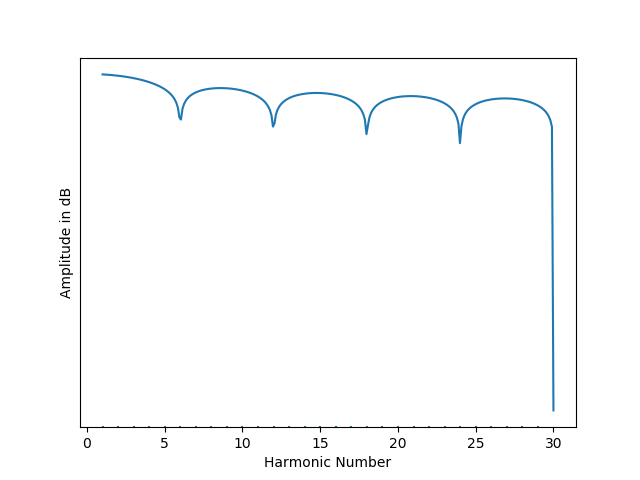
\includegraphics[scale=0.5]{theory.png}
\end{figure}

\section{Raw Guitar Analysis}

For the sake of thoroughness, with each parameter we change, we will measure the waveform created by the 'four corners' of the guitar fretboard. These are the open E strings, and same strings but freted at fret 12 (halfway along the string).

For the sake of brevity, we will pick the string at roughly the same location on the string.

The raw wavforms are shown below.
\begin{figure}[H]
\centering
\caption{Waveforms of Un-Amplified Electric Guitar}
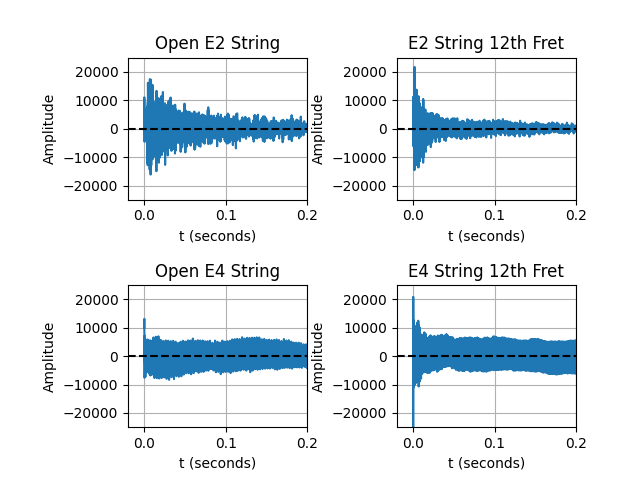
\includegraphics[scale=0.8]{raw_signal.png}
\end{figure}

Next we will take the Fourier transform of this wav data, using a fast-fourier transform method. We will also find the peaks. 

\begin{figure}[H]
\centering
\caption{Spectra of Un-Amplified Electric Guitar}
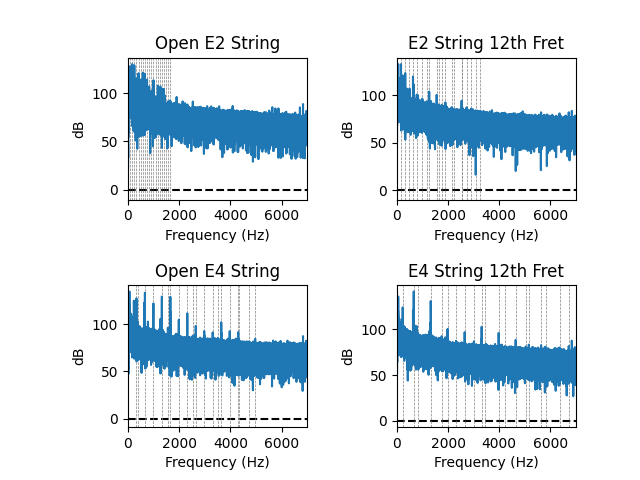
\includegraphics[scale=0.8]{fft_peaks.png}
\end{figure}

This is quite messy, so we will isolate the peaks from the wav data:

\begin{figure}[H]
\centering
\caption{Chopped Spectra of Un-Amplified Electric Guitar}
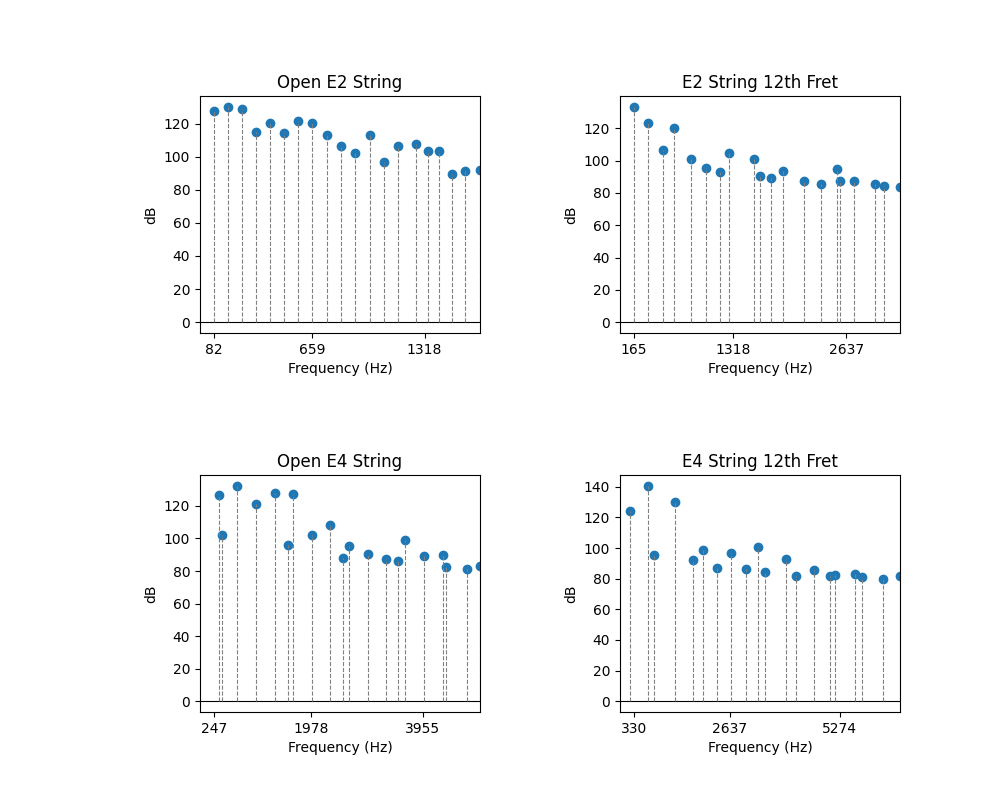
\includegraphics[scale=0.5]{ipeaks.png}
\end{figure}

Next, we connect these points. Furthermore, we segment each waveform by time slices. Now, we can see the time-evolution of the frequency spectrum.

\begin{figure}[H]
\centering
\caption{Spectra Evolution of Un-Amplified Electric Guitar}
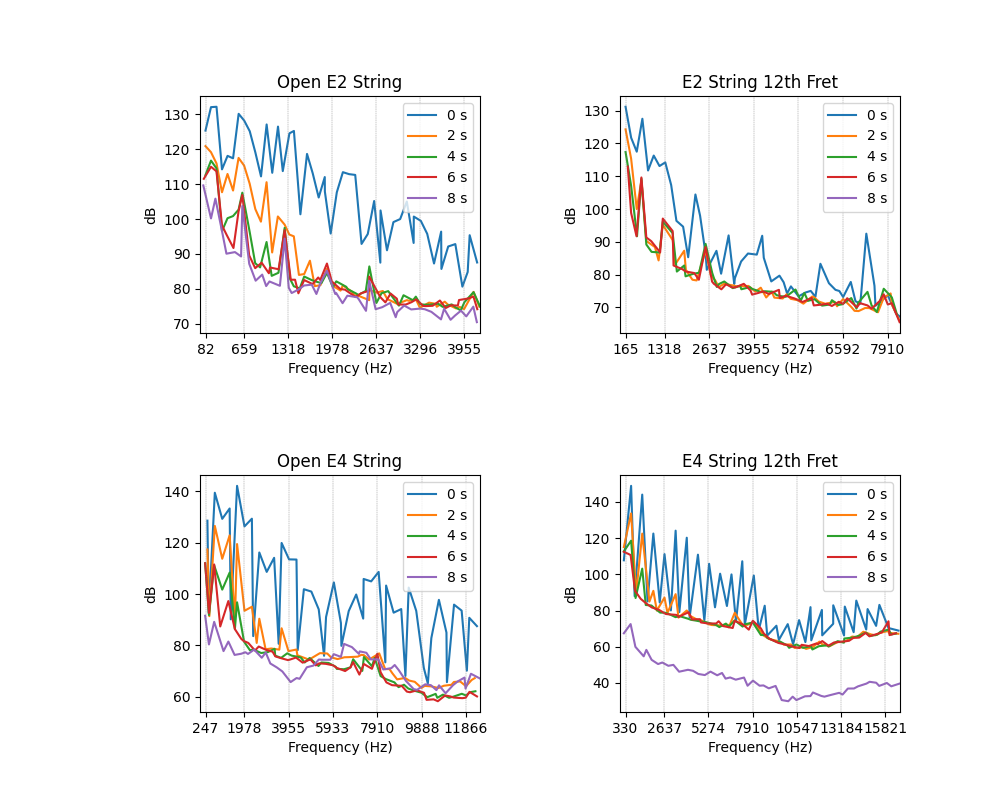
\includegraphics[scale=0.5]{rhvt.png}
\end{figure}

In this spectra evolution, the jagged pattern of the sinc function that we expect emerges slightly (particularly for the open E string).

In addition, it is also somewhat noticeable that the higher harmonics die off faster than those closer to the fundamental.
This makes sense as the damping of the instrument by the nut, bridge, and the string itself is proportional to velocity.
Therefore, lower harmonics are preserved relative to the higher ones.

\section{Plugging In}

Where things get exciting is when we plug the guitar into the amplifier unlocking a universe of controls to the tone of the guitar.

\subsection{'Clean Signal'}

There are many particular qualities of the electronics in the amplifier
, so the effects that changing the electronic signal of the guitar should be observed relative to a clean signal.

The spectra evolution of the clean signal is shown here:

\begin{figure}[H]
\centering
\caption{Spectra Evolution of Clean, Amplified Electric Guitar}
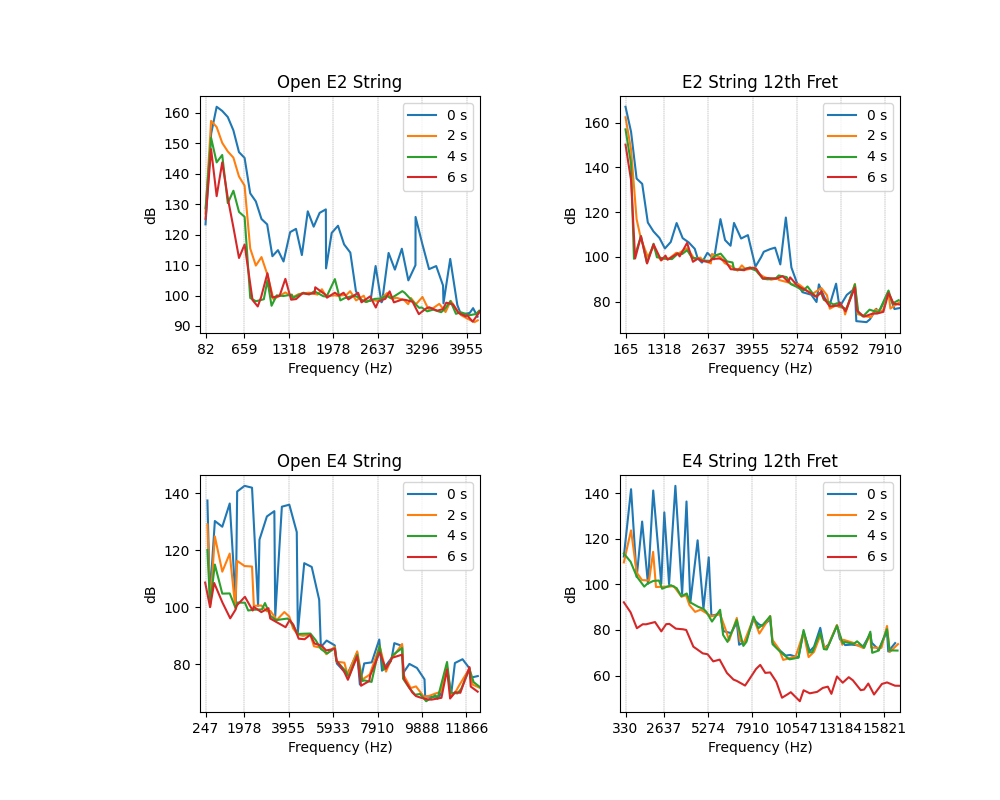
\includegraphics[scale=0.5]{clean_hvt.png}
\end{figure}

Again, one must not take too much from this measurement, as the basic tone settings for this amplifier may prioritize the lower harmonics for example. However, it is good to see the jagged amplitude function as well as the quick decay of the higher harmonics again.

We are using the bridge pickup for the rest of the measurements (again for the sake of brevity).

\subsection{Using the Tone Knob}
One of the first controls available for the guitar's tone is the tone knob. 
The tone knob is a pontentiometer in a resistive-capacitive low-pass filter. Increasing the resistance of the potentiometer increases the influence of the RC circuit, thereby diminishing the higher harmonics of the spectra of the signals.

The following is the spectra evolution of the clean signal, but instead of the low-pass filter having as little influence as possible (dial turned to 10), the dial is turned to 1 -- decreasing the cut-off frequency of the filter.


\begin{figure}[H]
\centering
\caption{Spectra Evolution of Rolled-Off Electric Guitar}
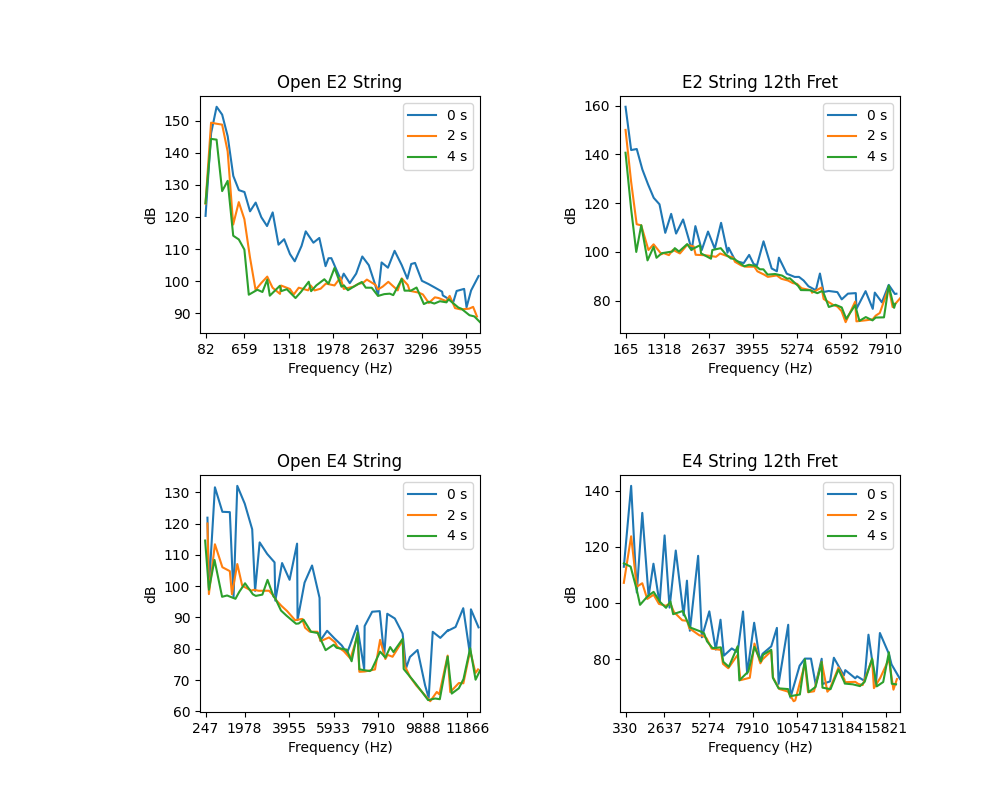
\includegraphics[scale=0.5]{rolhvt.png}
\end{figure}

Admittedly, the effects are sublte. We are looking for a decrease/steepening in average slope of the spectra. This is slightly visible in the open high E string.

\subsection{Using Compression}
Another basic electric guitar control is the compression.
the signal entering a compressor circuit is split between a voltage-control amplifier and what is called a 'side-chain.'

Note, this is again with maximal tone on the guitar to make the higher harmonics as visible as possible.

\begin{figure}[H]
\centering
\caption{Spectra Evolution of Compressed Electric Guitar}
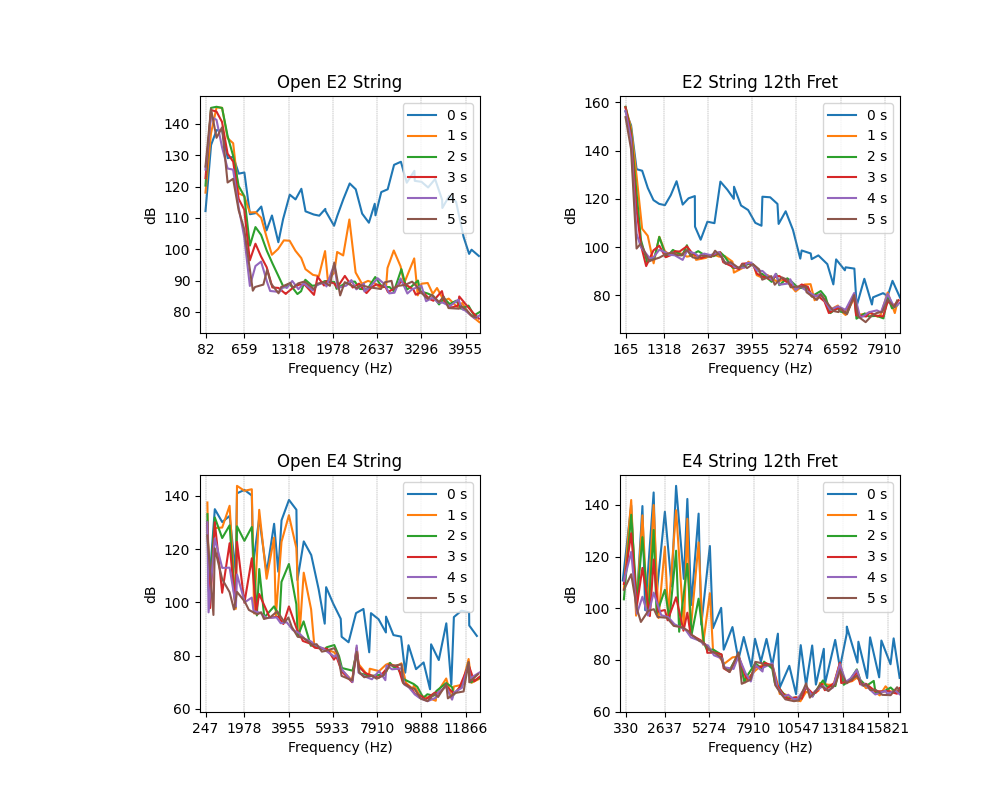
\includegraphics[scale=0.5]{comphvt.png}
\end{figure}

\subsection{Using Overdrive}
Lastly, we will visualize the effects of overdrive on the guitar signal.
Overdrive circuits mainly use diode loops in the feedback loop of operational amplifiers to 'soft-clip' the guitar signal.
Clipping a waveform in this way, naturally introduces more harmonics to the Fourier series, as it turns something like a sin wave into more of a square wave.
The same is true with a complex guitar signal; clipping its peaks and troughs introduces more harmonics into the picture.

\begin{figure}[H]
\centering
\caption{Spectra Evolution of Overdriven Electric Guitar}
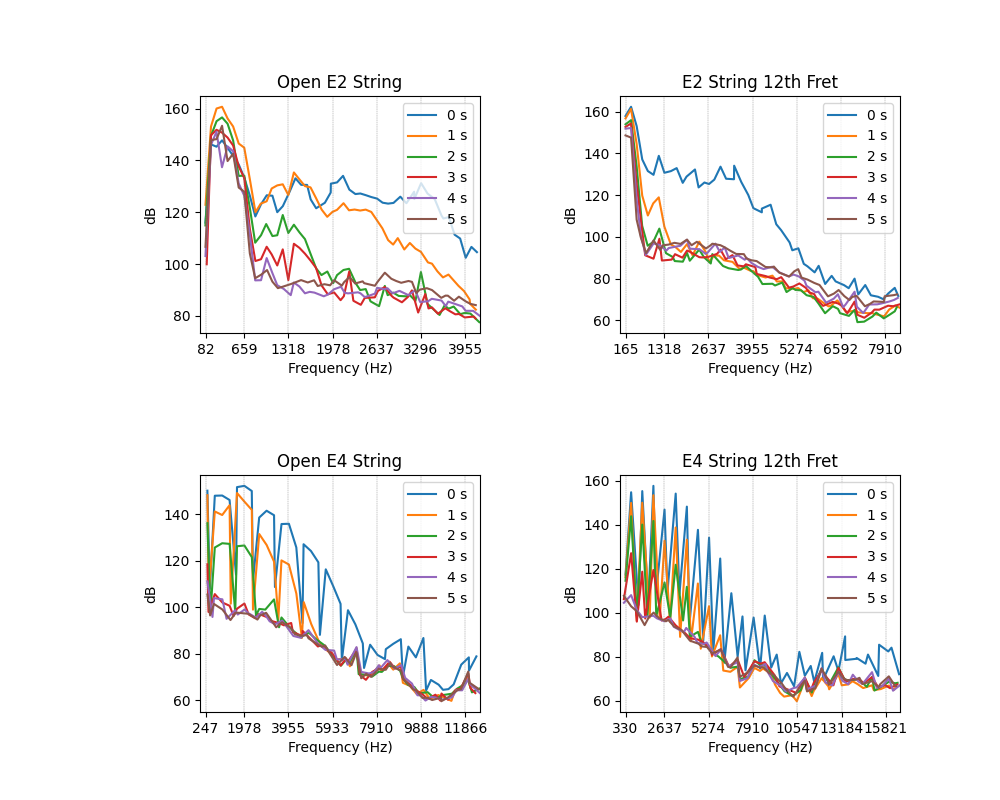
\includegraphics[scale=0.5]{odhvt.png}
\end{figure}

\section{Conclusion}

Hopefully, with this report, we have successfully illustrated the effects that electric guitar controls (that are characteristic of being electric -- not acoustic) have on the frequency spectrum of their output.
The wav files recorded seem to have been very noisy, thereby blurring the clarity of the harmonics, but the spectra have overall been shaped appropriately by the controls.

\end{document}
